%%%%%%%%%%%%%%%%%%%%%%%%%%%%%%%%%%%%%%
\chapter{Signal modeling and statistical treatment}
\label{ch:sigModel}
%%%%%%%%%%%%%%%%%%%%%%%%%%%%%%%%%%%%%%

%%%%%%%%%%%%%%%%%%%%%%%%%%%%%%%%%%%%%%
\section{Signal modeling}
 \subsection{Parametrization of the resonance mass}

 \begin{figure}[htbp]
 \centering
 \begin{tabular}{cc}
 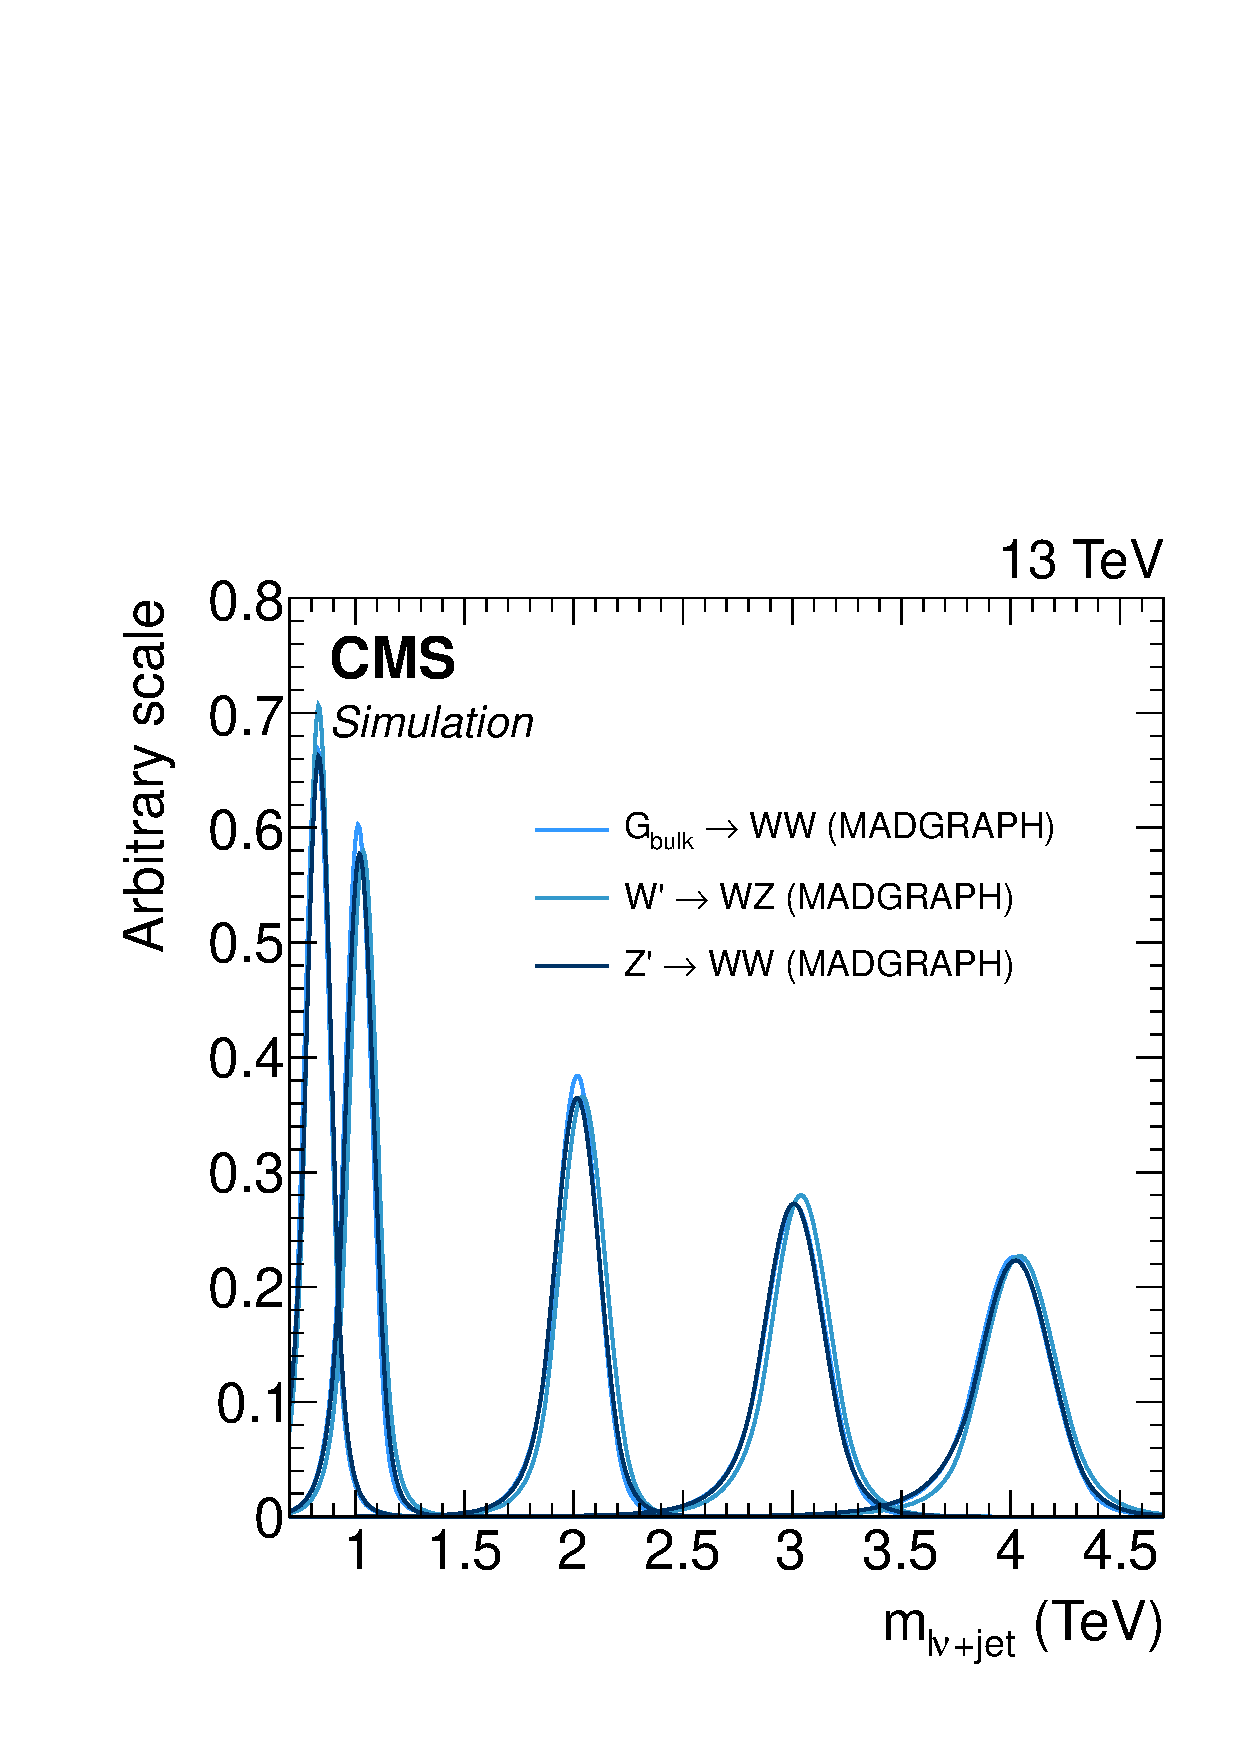
\includegraphics[width=0.48\textwidth]{\chten/WVanalysis/line-shapes-mlvj}
 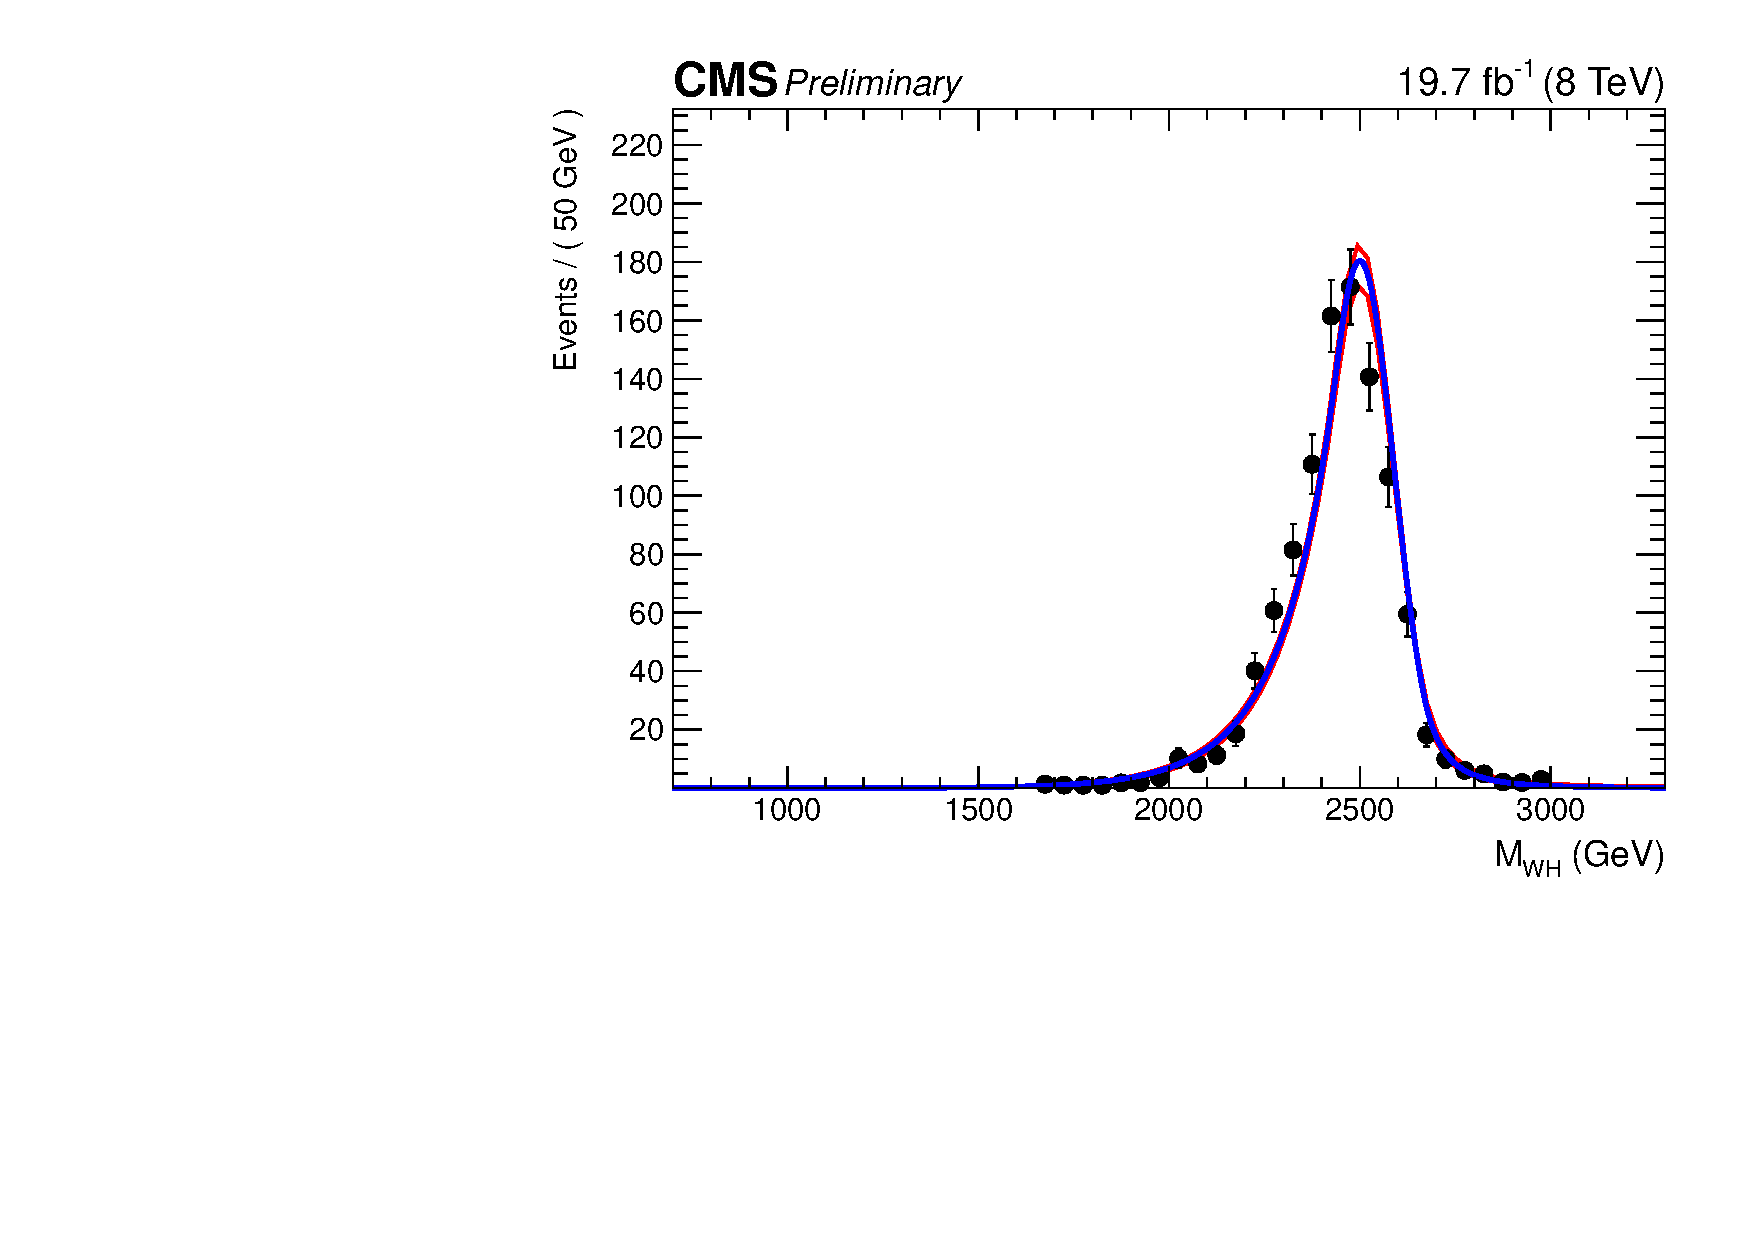
\includegraphics[width=0.48\textwidth]{\chten/WHanalysis/DCBfits/mu/treeEDBR_MWp_2500_bb_xwh_mu_m_lvj_signal_regionDoubleCB_v1.pdf} 
 \end{tabular}
 \caption{ml?+jet (right) distribution for different signal mass hypotheses used to extract the signal shape.}
 \label{fig:signalModel}
 \end{figure} 

%%%%%%%%%%%%%%%%%%%%%%%%%%%%%%%%%%%%%%
\subsection{Signal efficiency}

\begin{figure}[htb]
\centering
\begin{tabular}{lr}
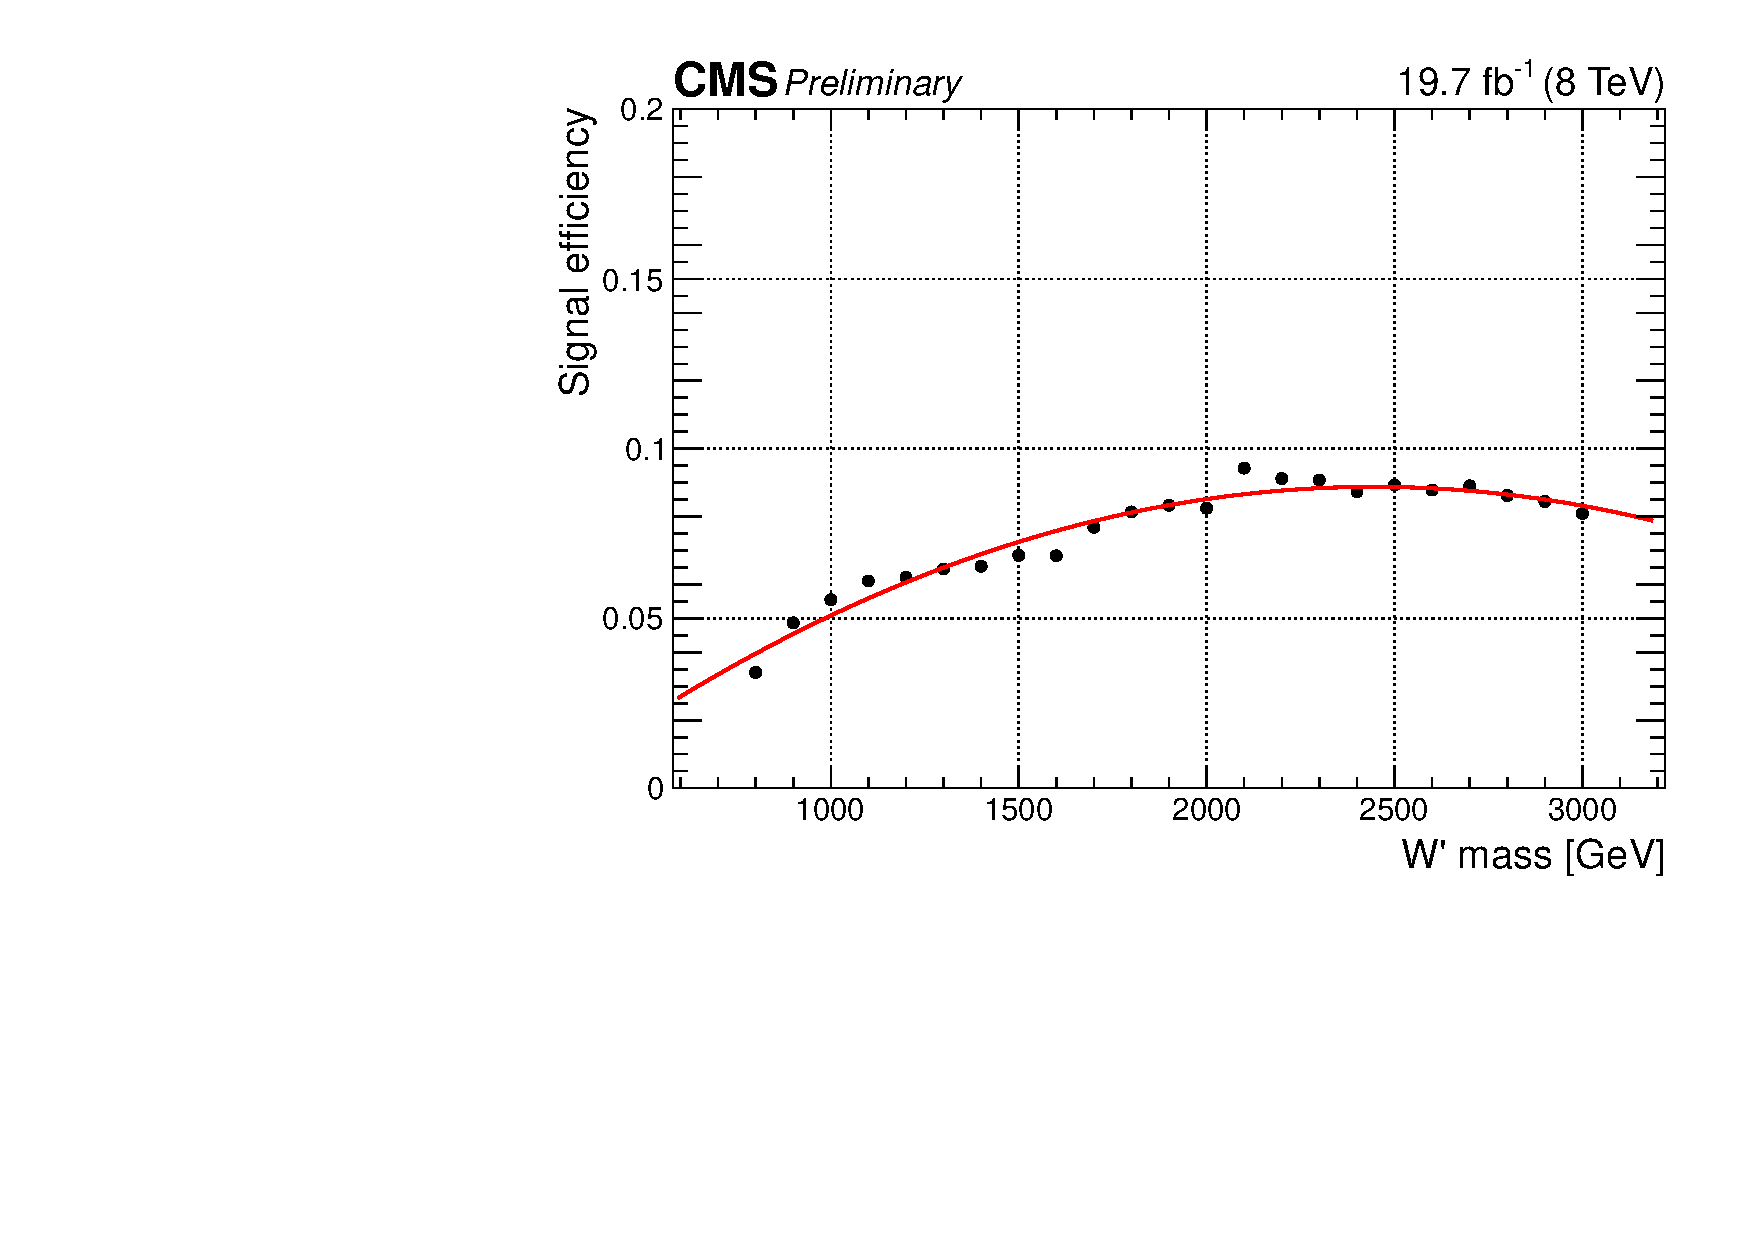
\includegraphics[width=0.5\textwidth]{\chten/WHanalysis/signalEff_mu.pdf} &
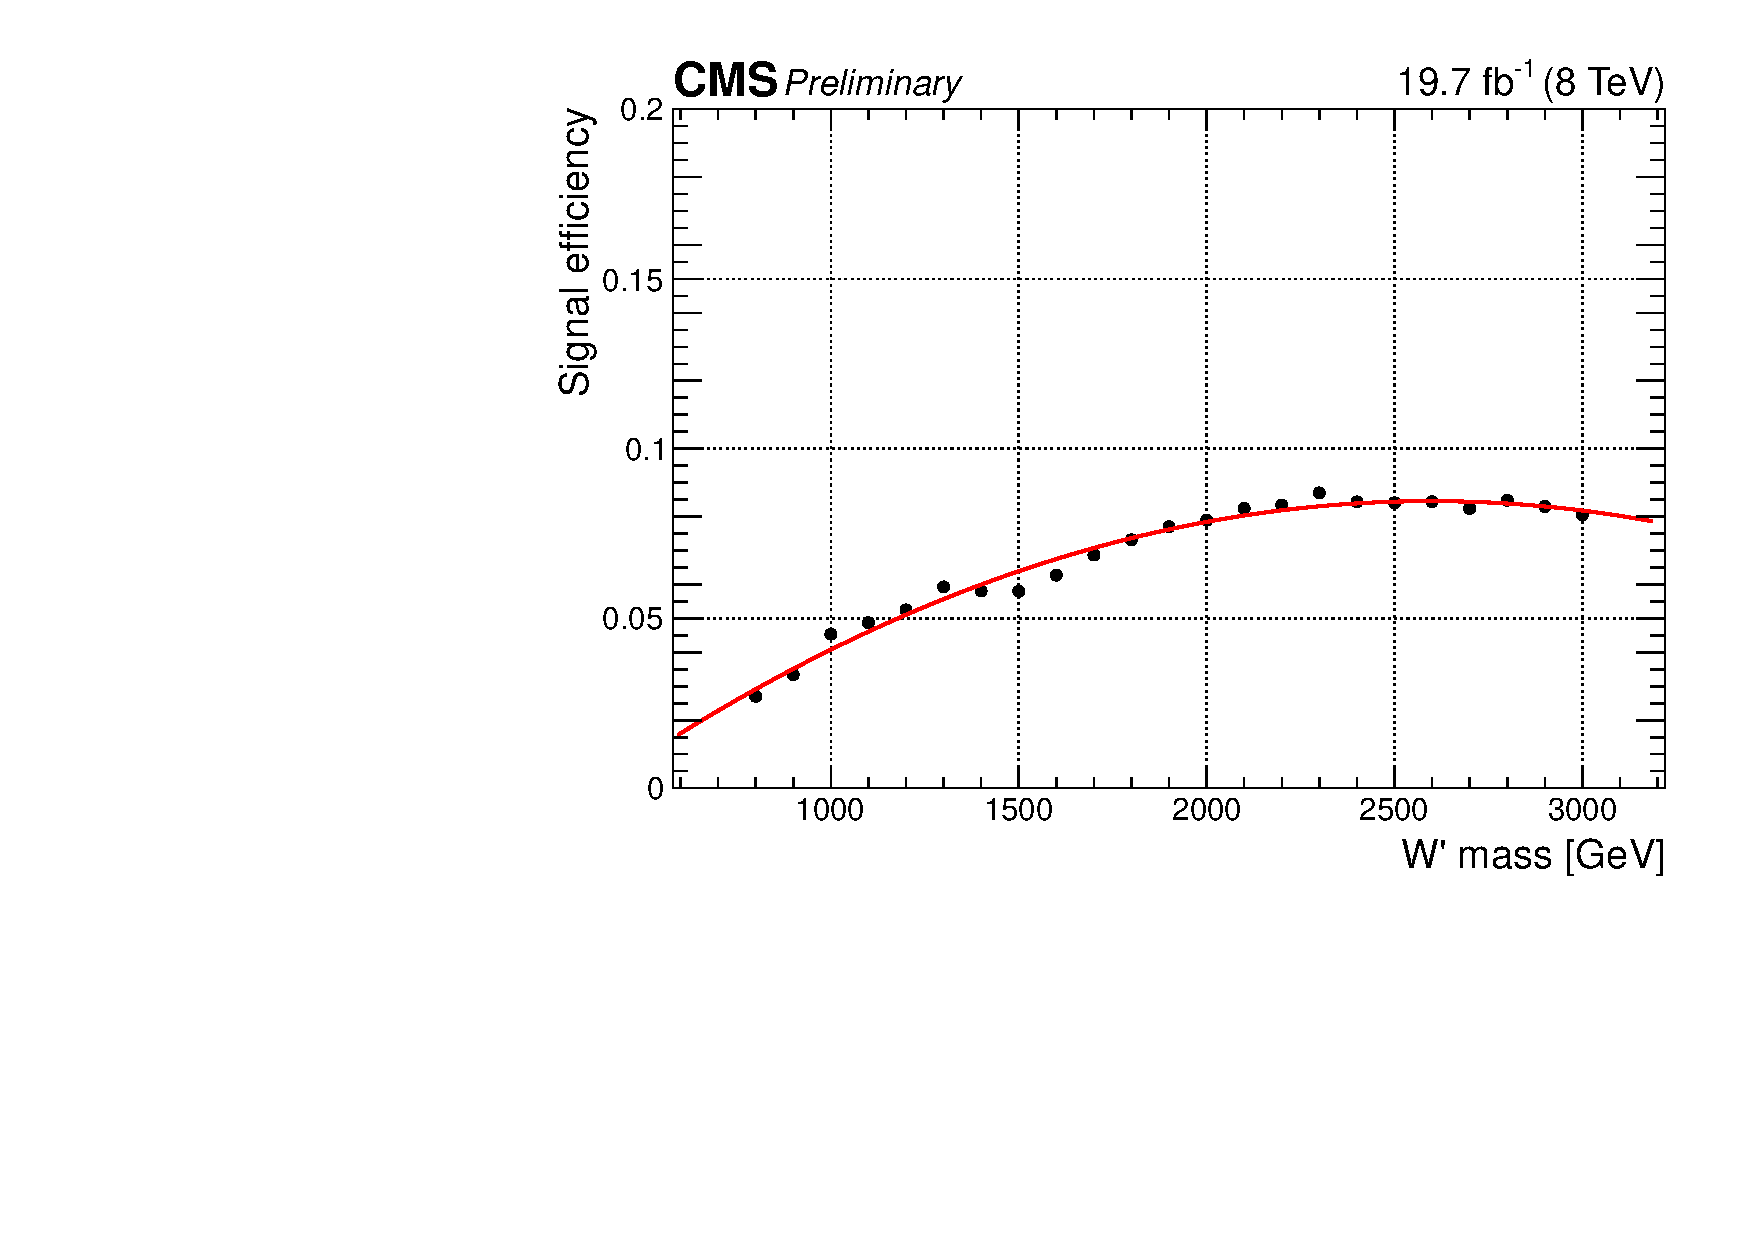
\includegraphics[width=0.5\textwidth]{\chten/WHanalysis/signalEff_ele.pdf} \\
\end{tabular}
\caption{Signal efficiency for the final selection criteria as a function of the $\PWpr$ mass hypothesis in the muon (left) and electron (right) channel.}
\label{fig:signalEff}
\end{figure}

\begin{figure}[htbp]
\centering
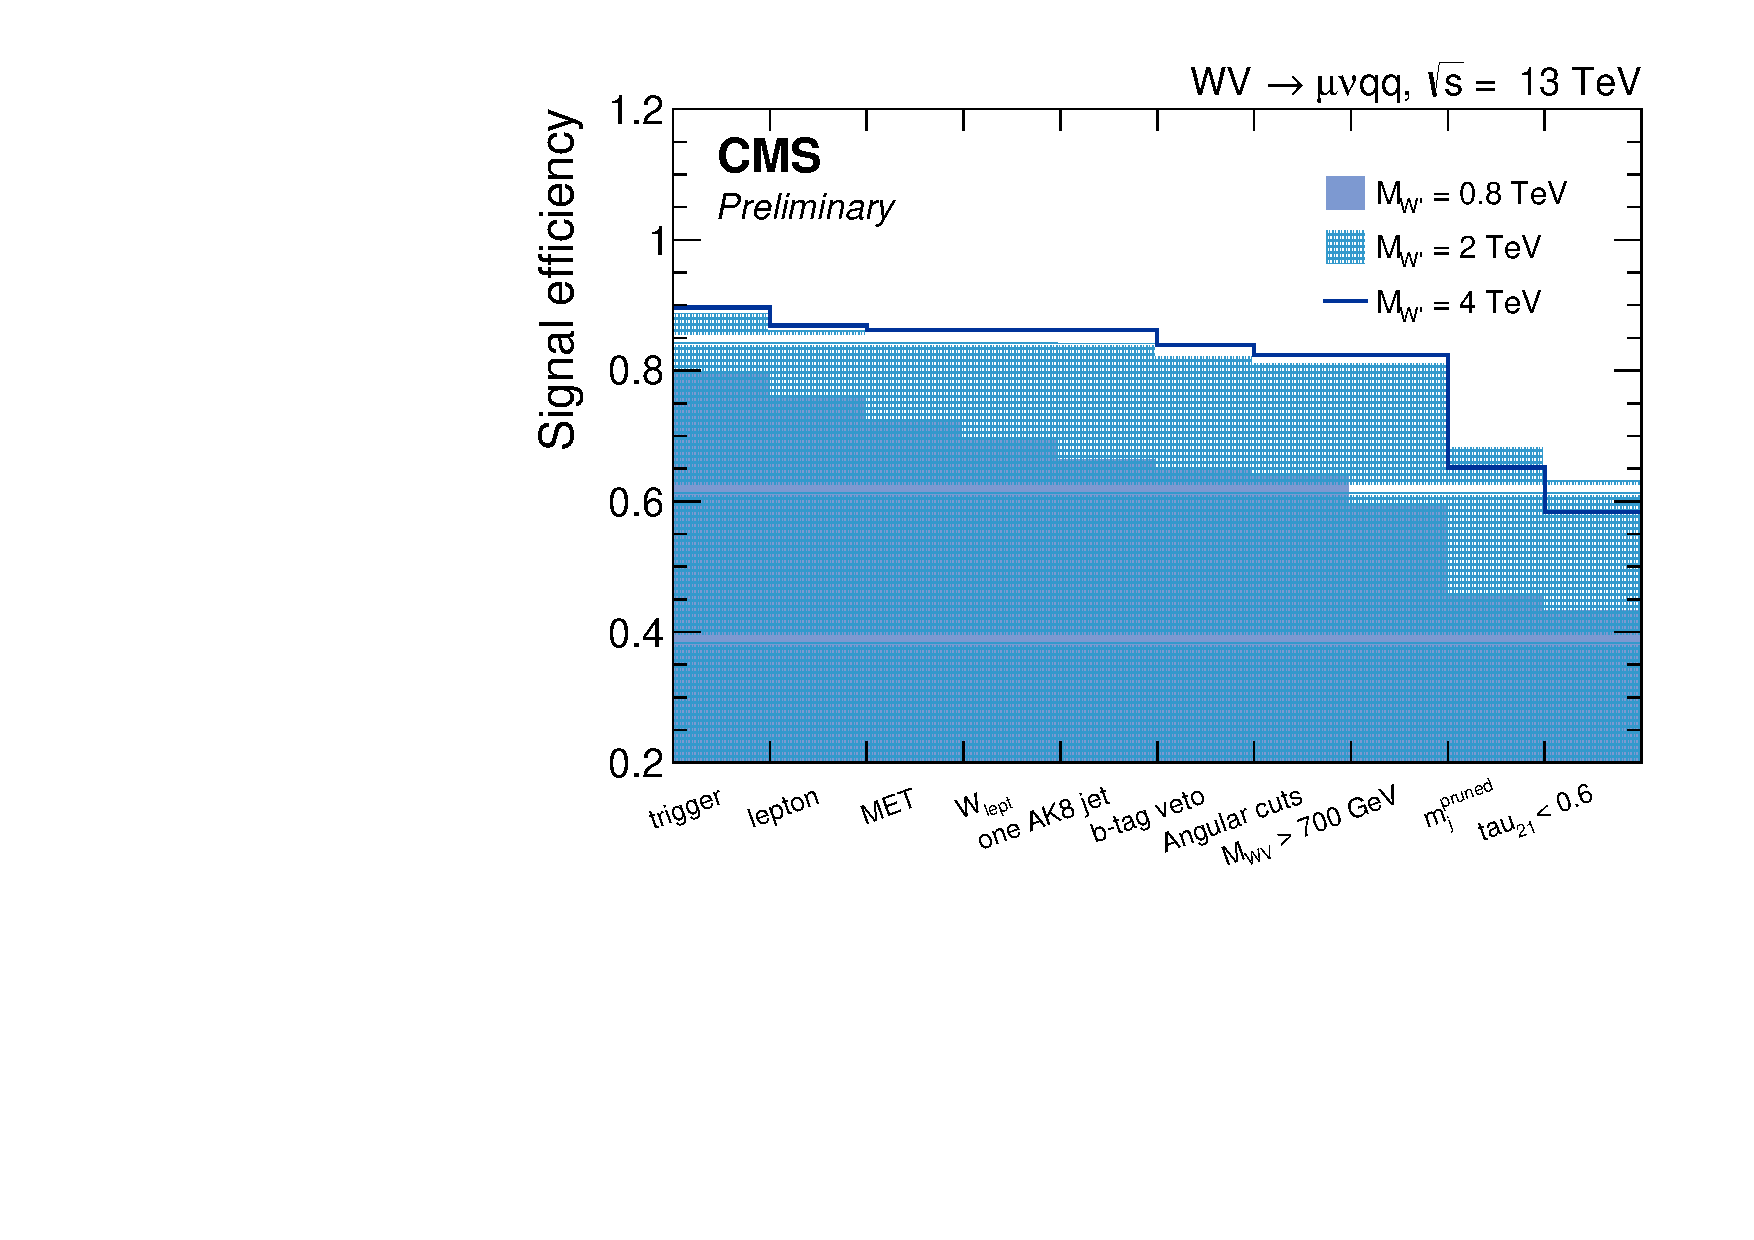
\includegraphics[width=0.48\textwidth]{\chten/WVanalysis/SignalEff/eff_wpall_wp_mu.pdf}%
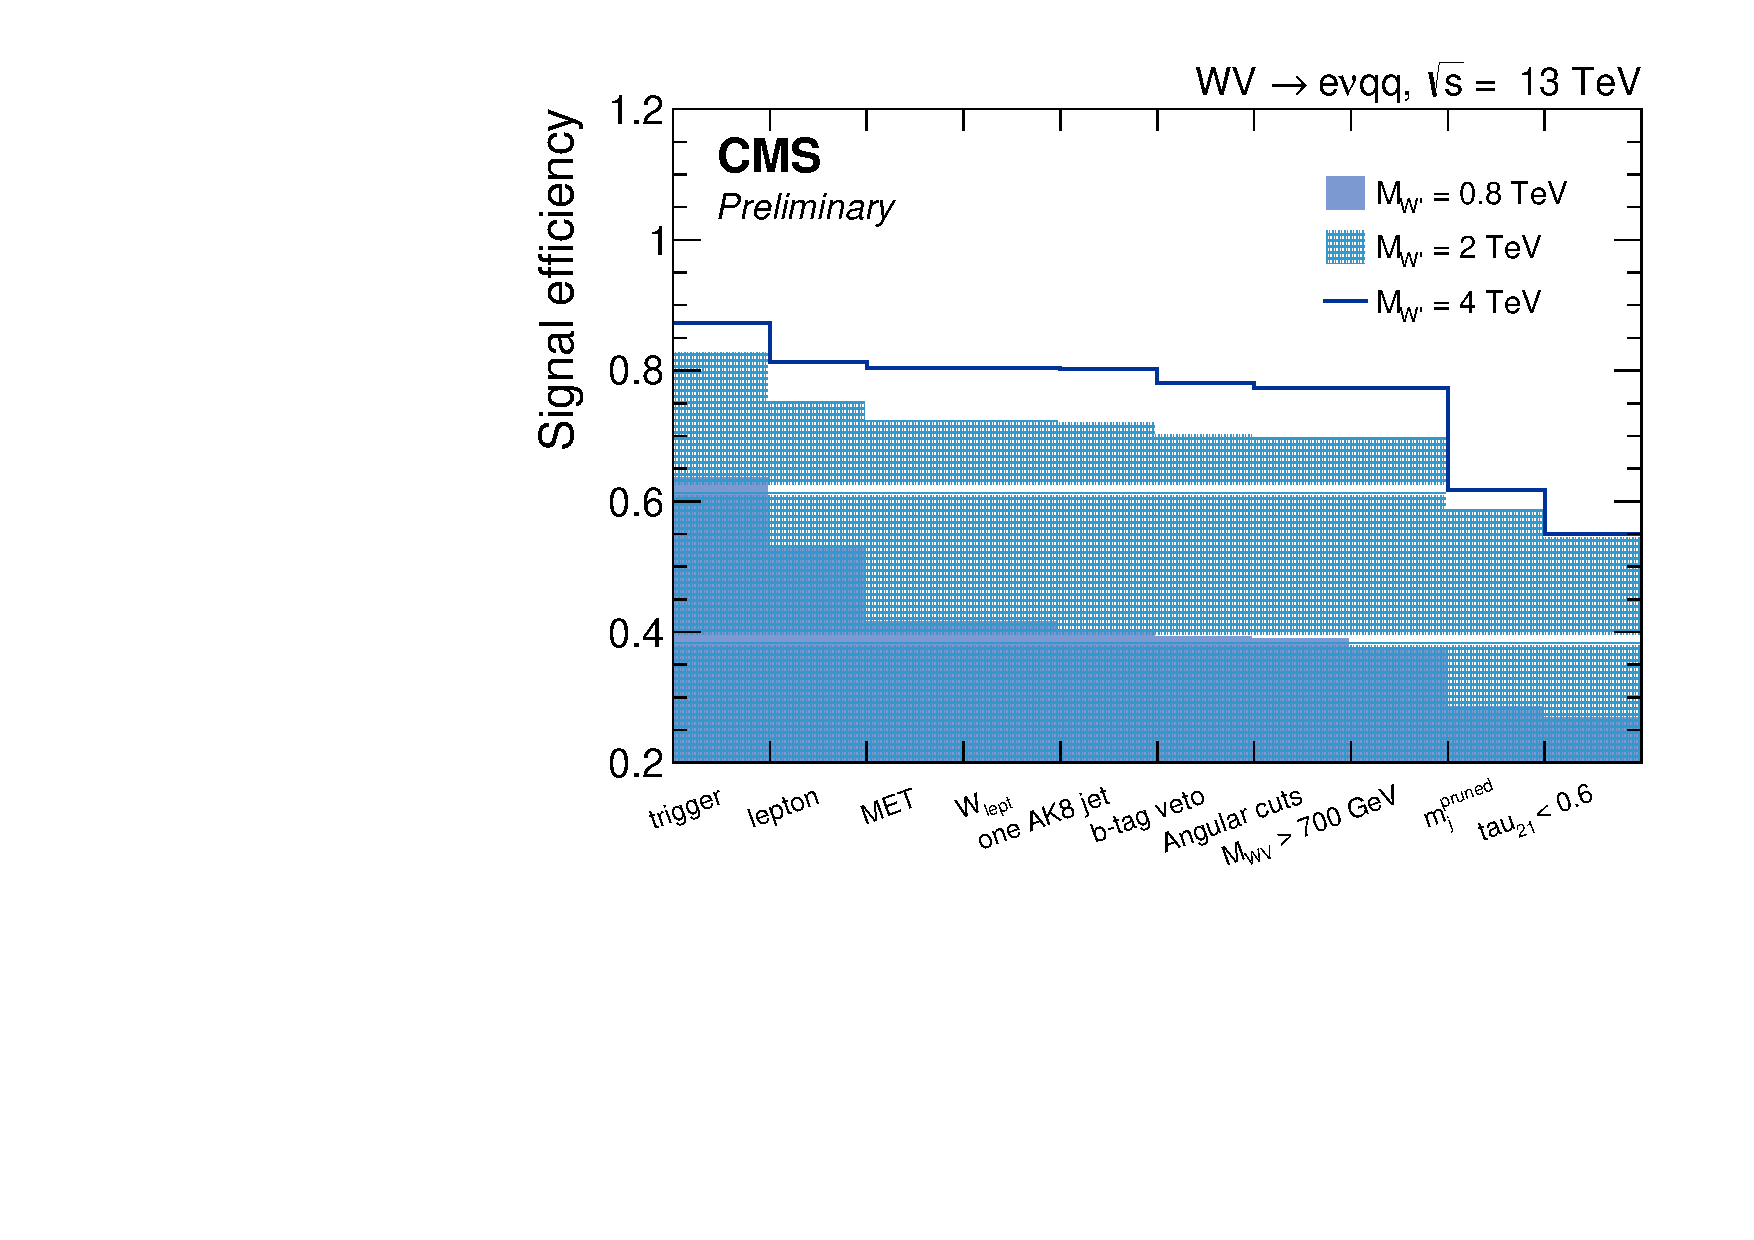
\includegraphics[width=0.48\textwidth]{\chten/WVanalysis/SignalEff/eff_wpall_wp_el.pdf}\\
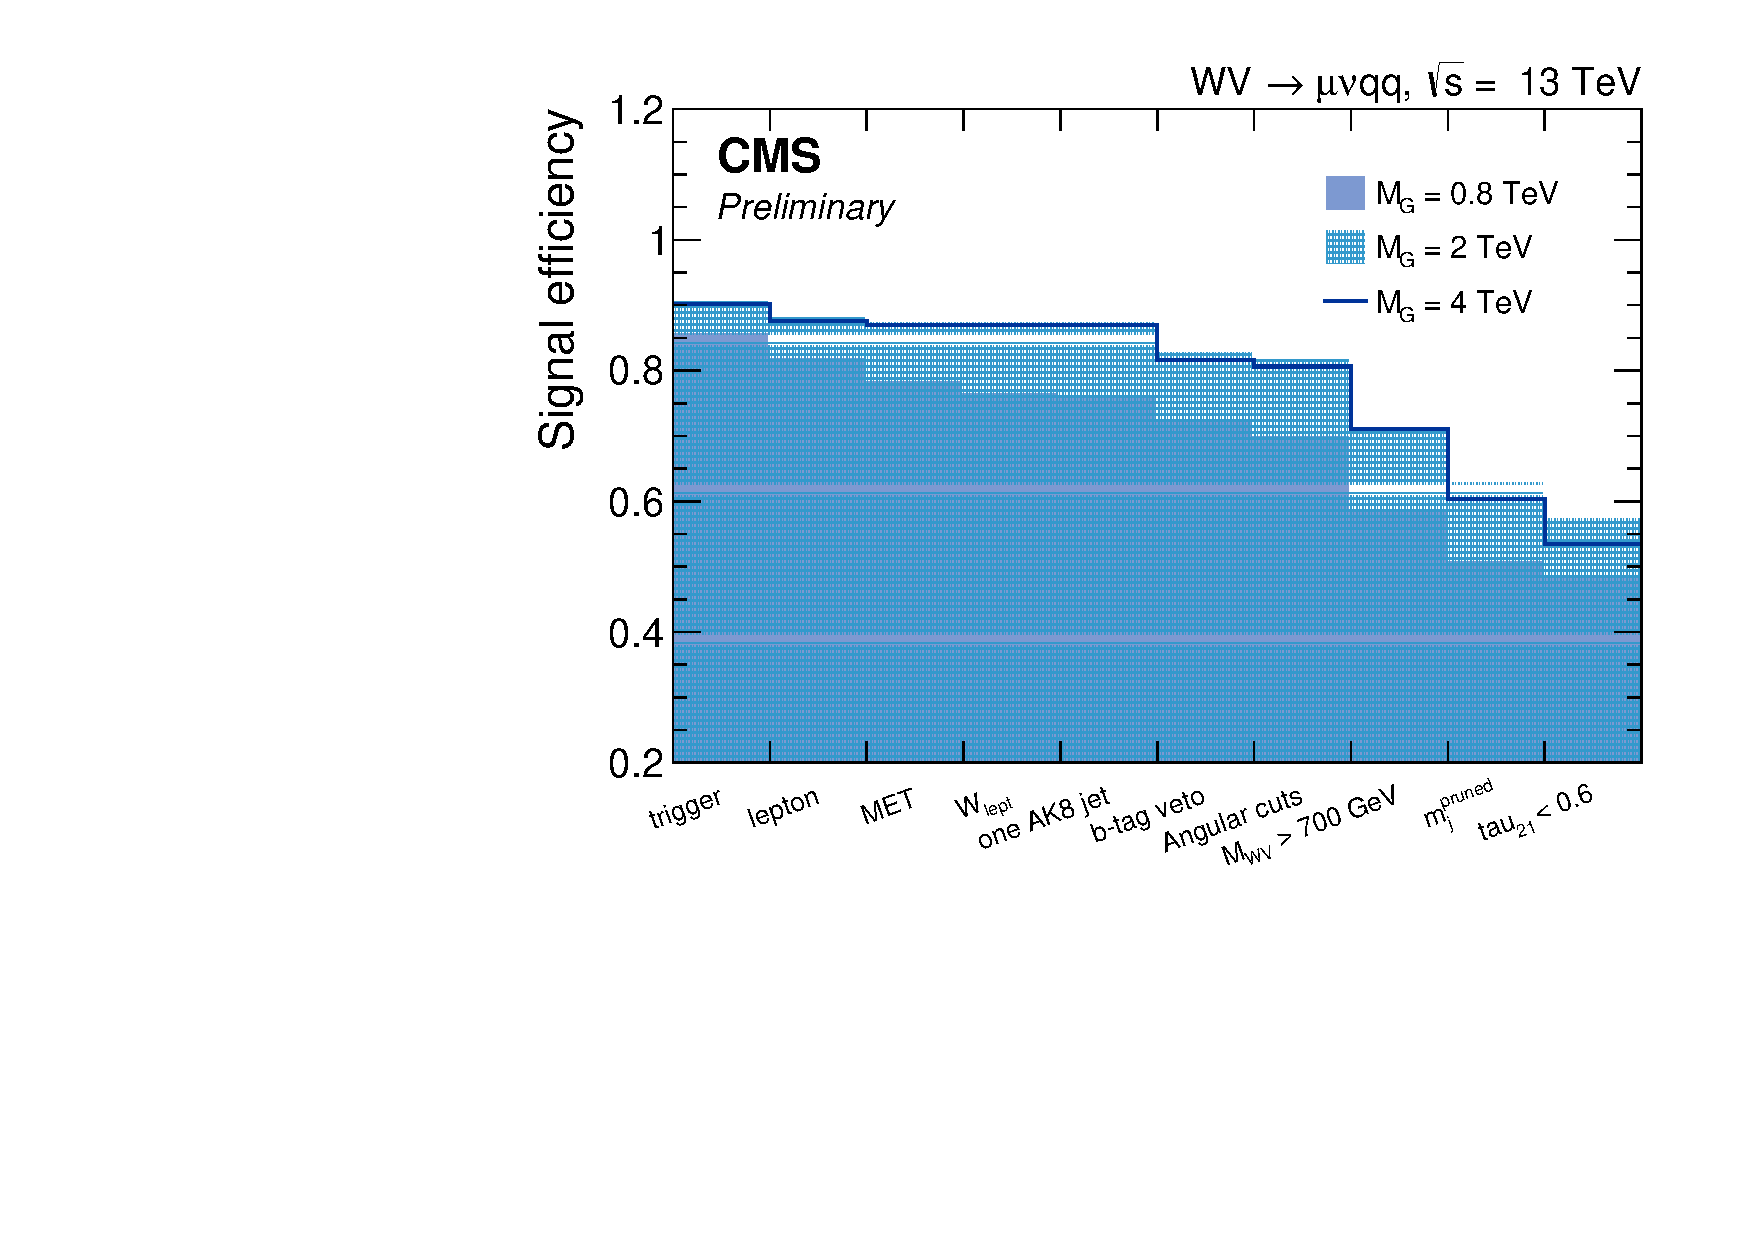
\includegraphics[width=0.48\textwidth]{\chten/WVanalysis/SignalEff/eff_gall_g_mu.pdf}
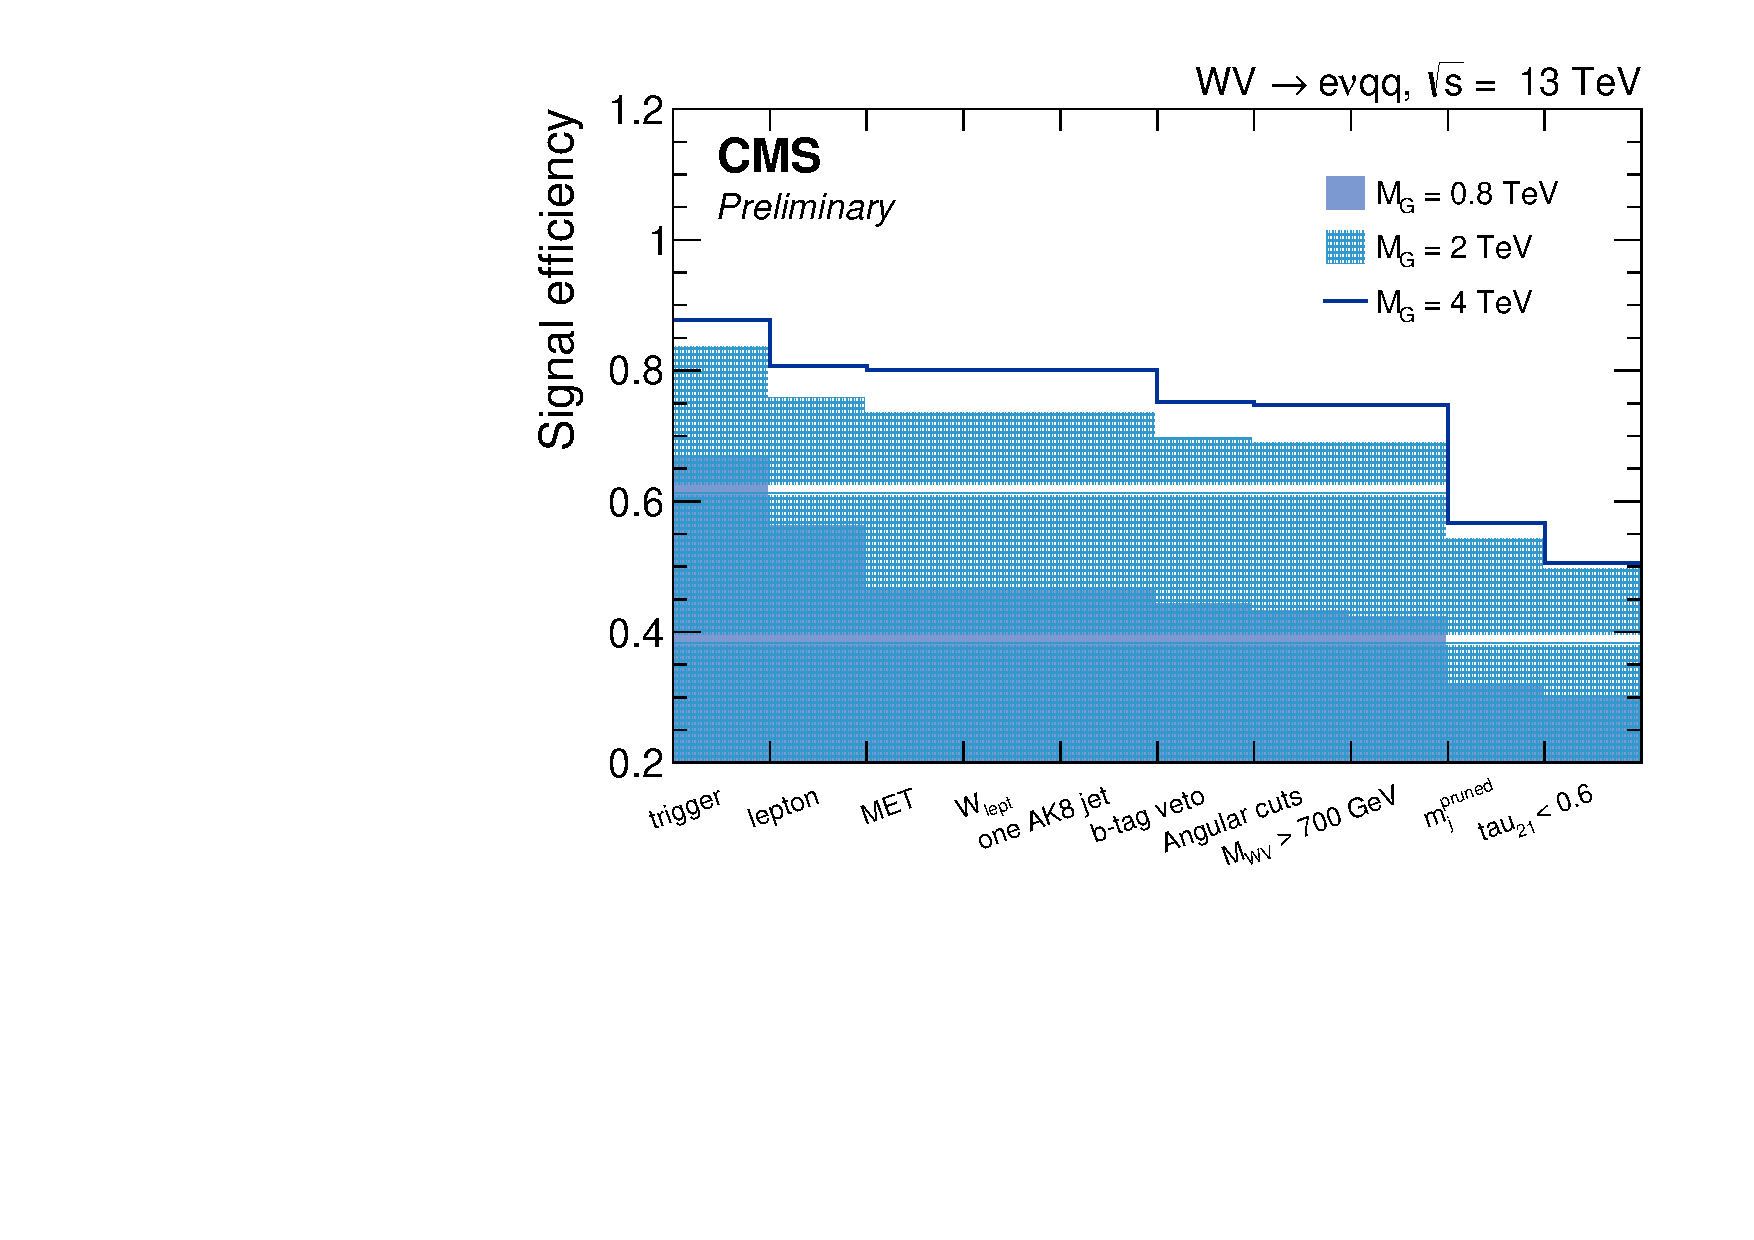
\includegraphics[width=0.48\textwidth]{\chten/WVanalysis/SignalEff/eff_gall_g_el.pdf}\\
\caption{Expected signal efficiency of each selection in the muon (left) and electron (right) channels
for 3 mass points, for W' (top) and BulkG (bottom) signal models.}
\label{fig:sigcutflow}
\end{figure}

\begin{figure}[htbp]
\centering
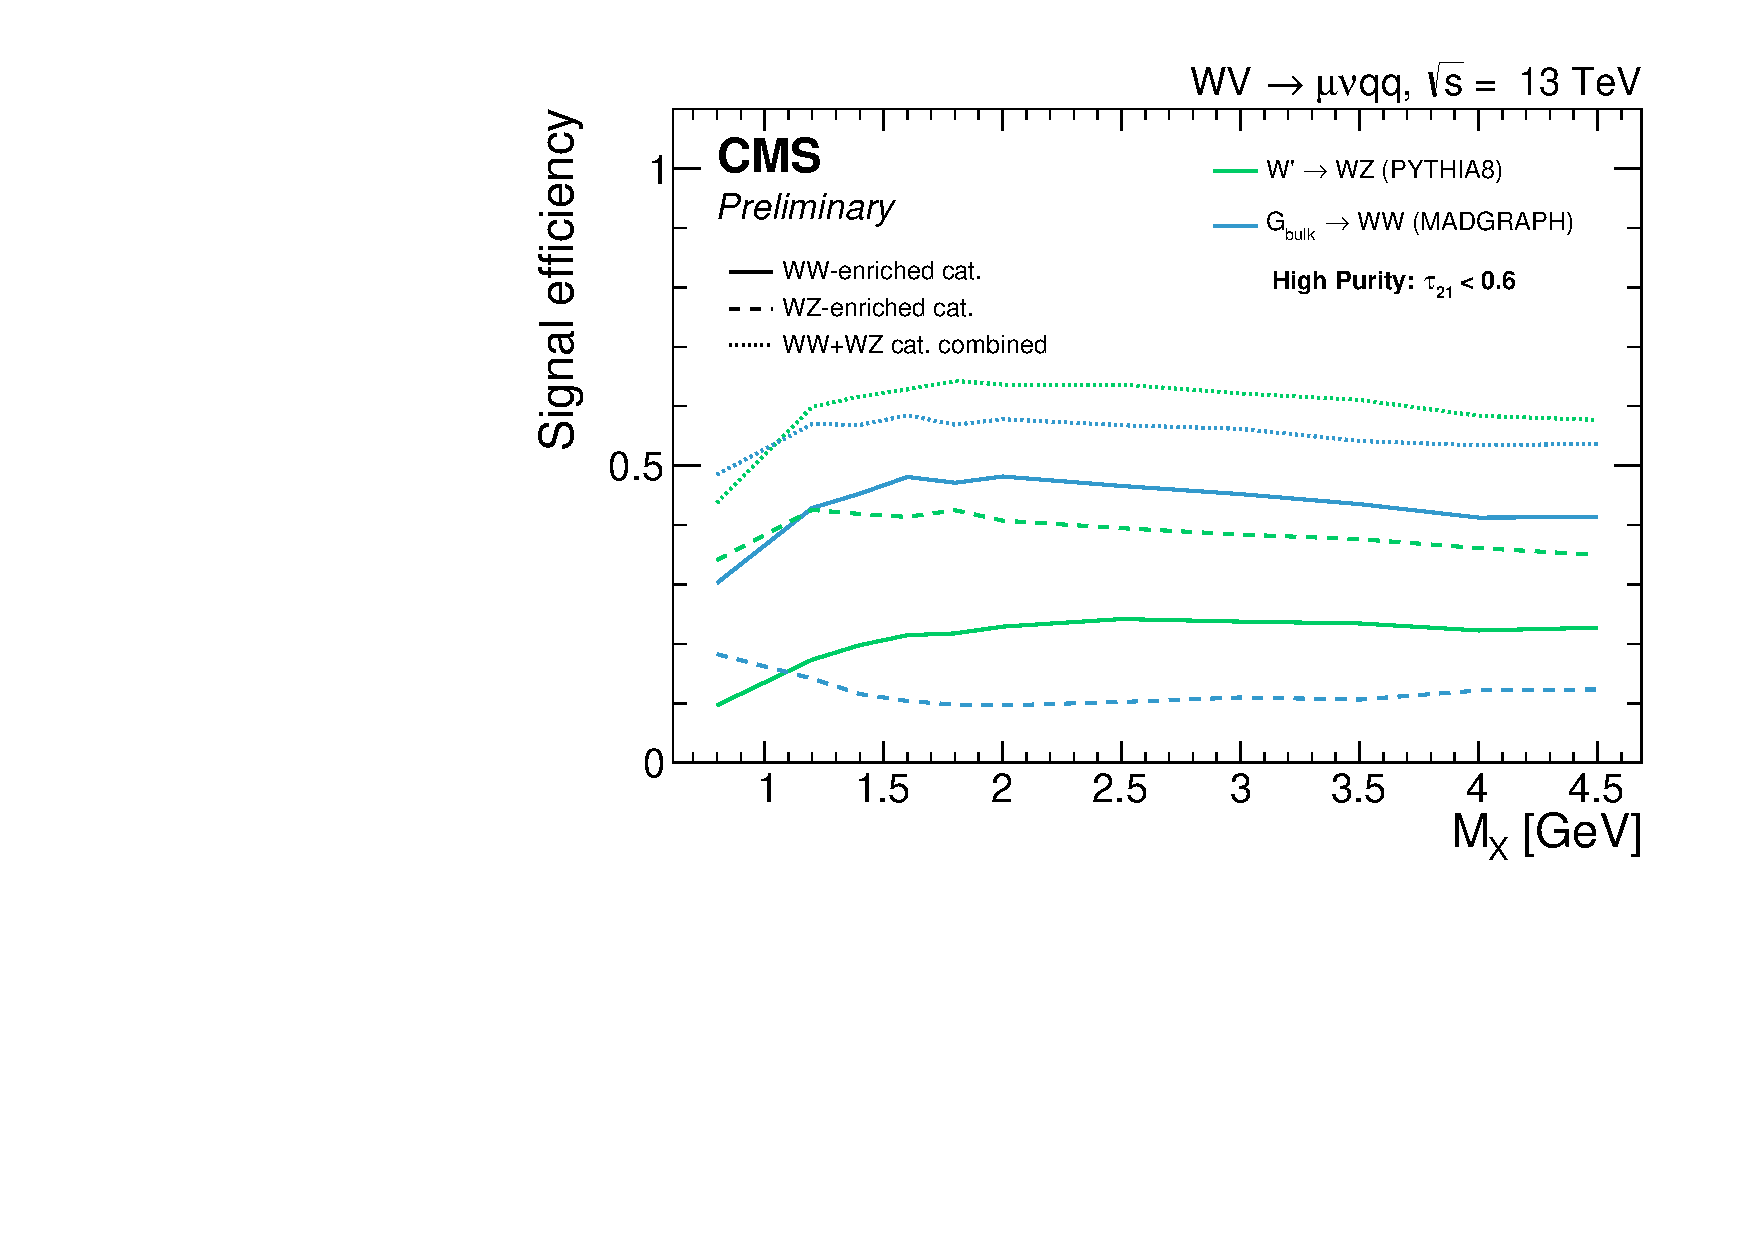
\includegraphics[width=0.48\textwidth]{\chten/WVanalysis/SignalEff/eff_HPV_mu.pdf}%
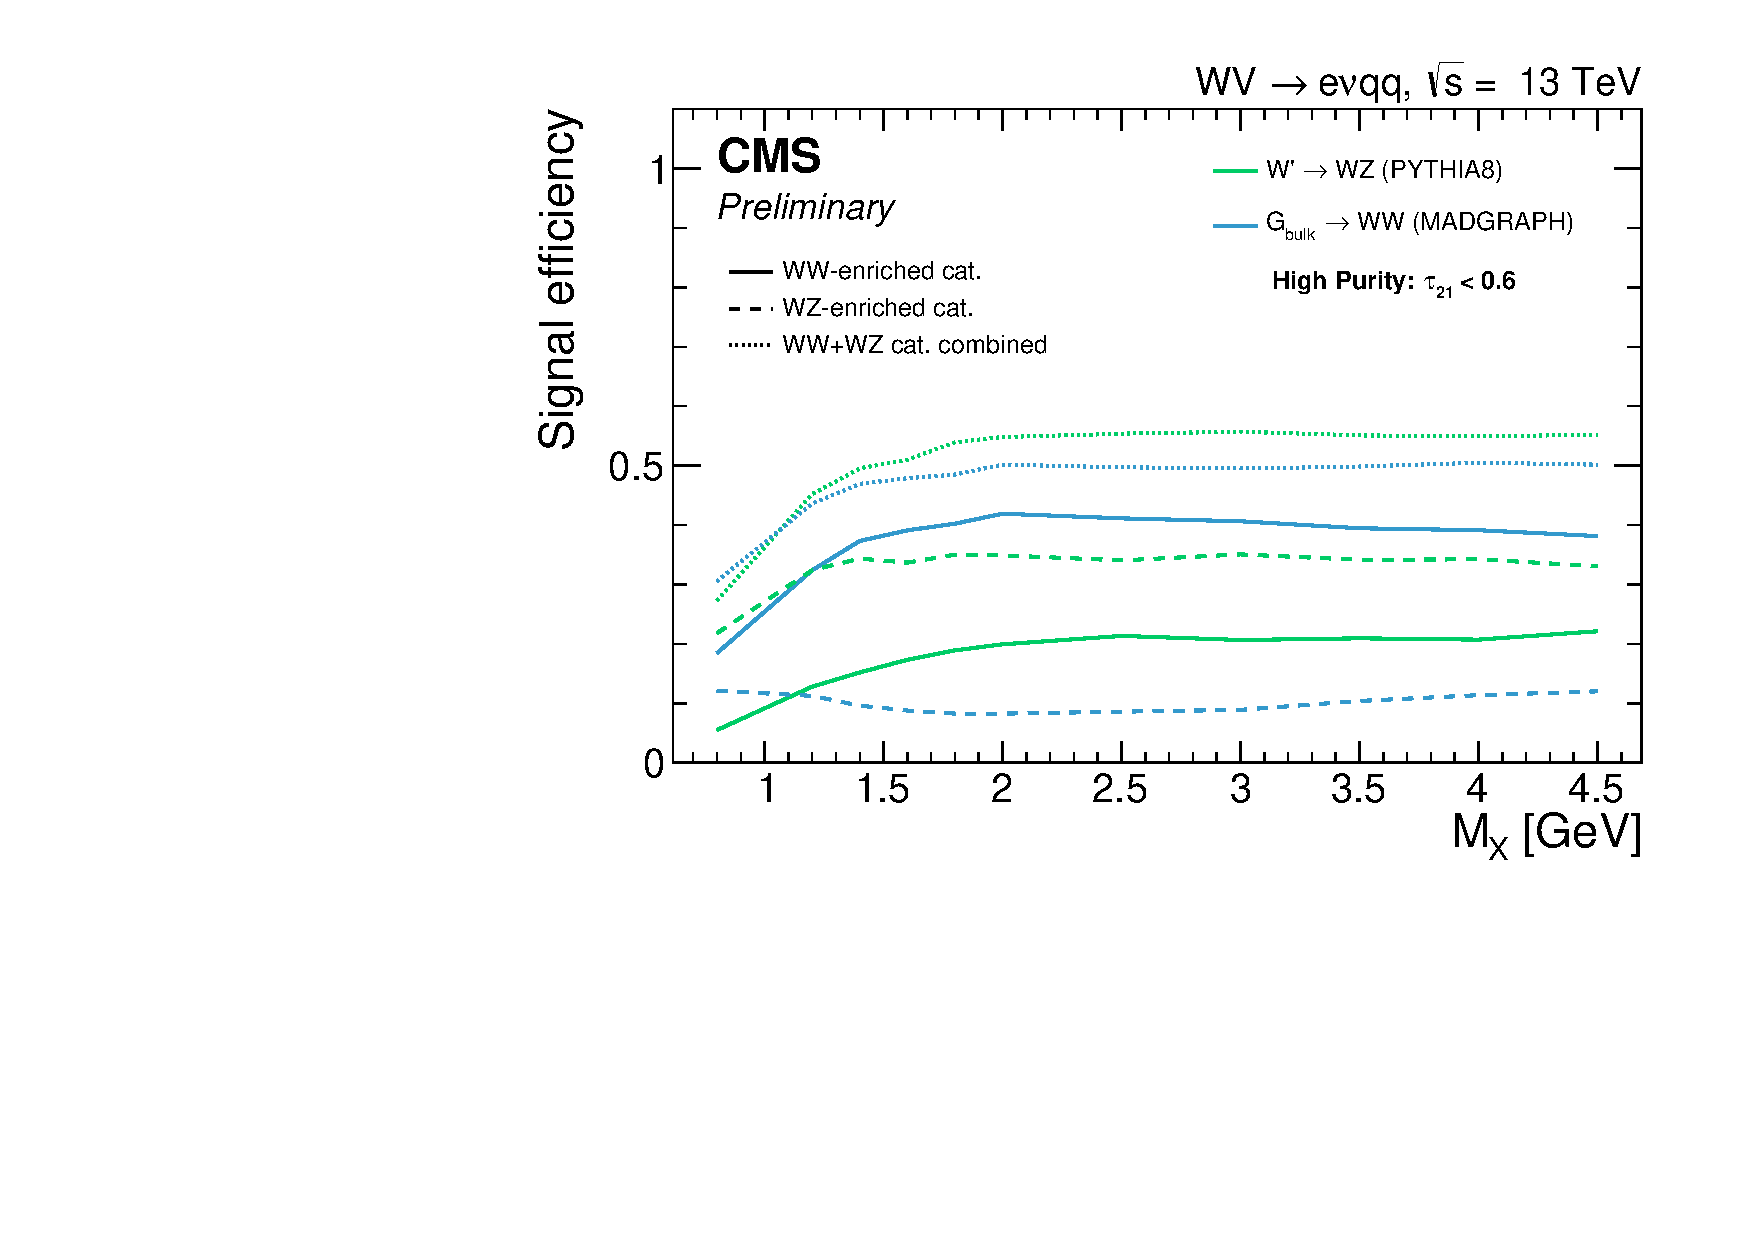
\includegraphics[width=0.48\textwidth]{\chten/WVanalysis/SignalEff/eff_HPV_el.pdf}\\
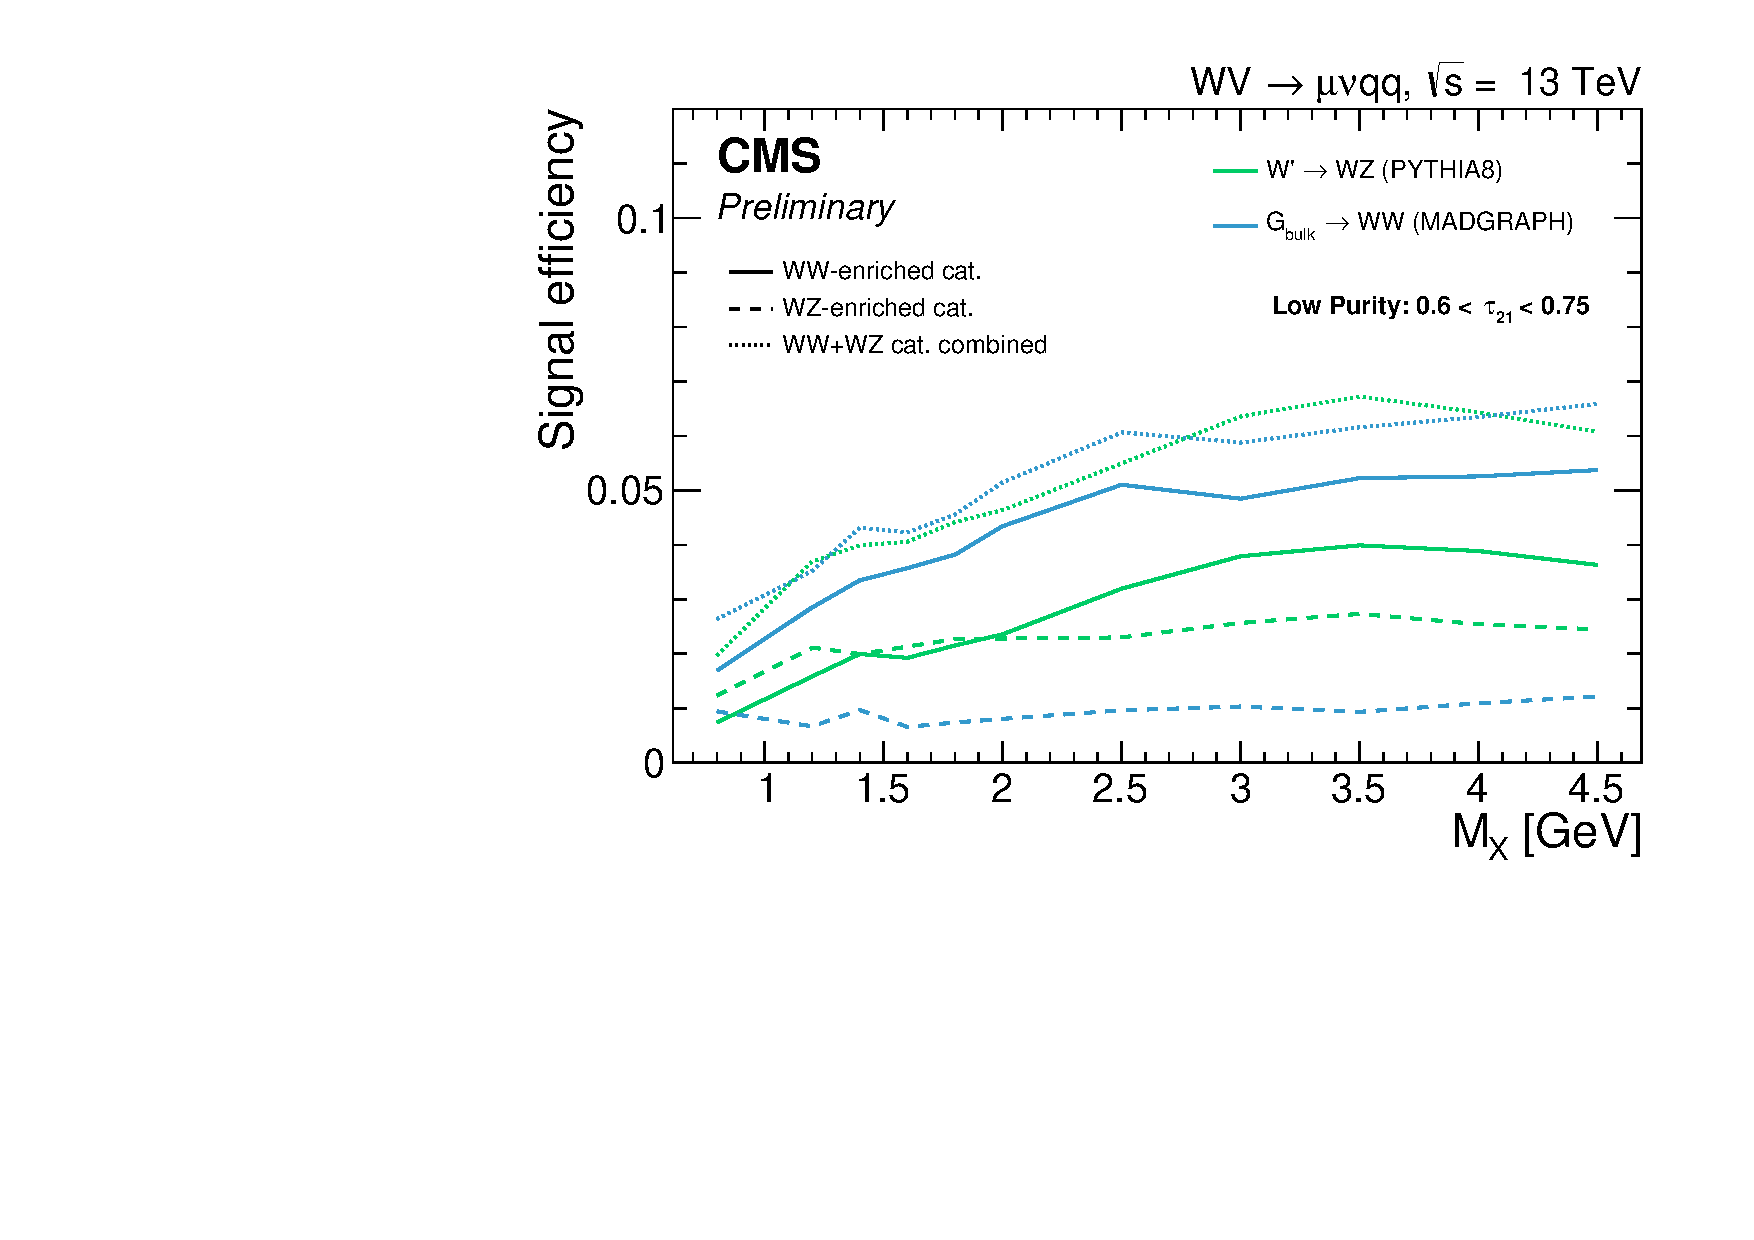
\includegraphics[width=0.48\textwidth]{\chten/WVanalysis/SignalEff/eff_LPV_mu.pdf}
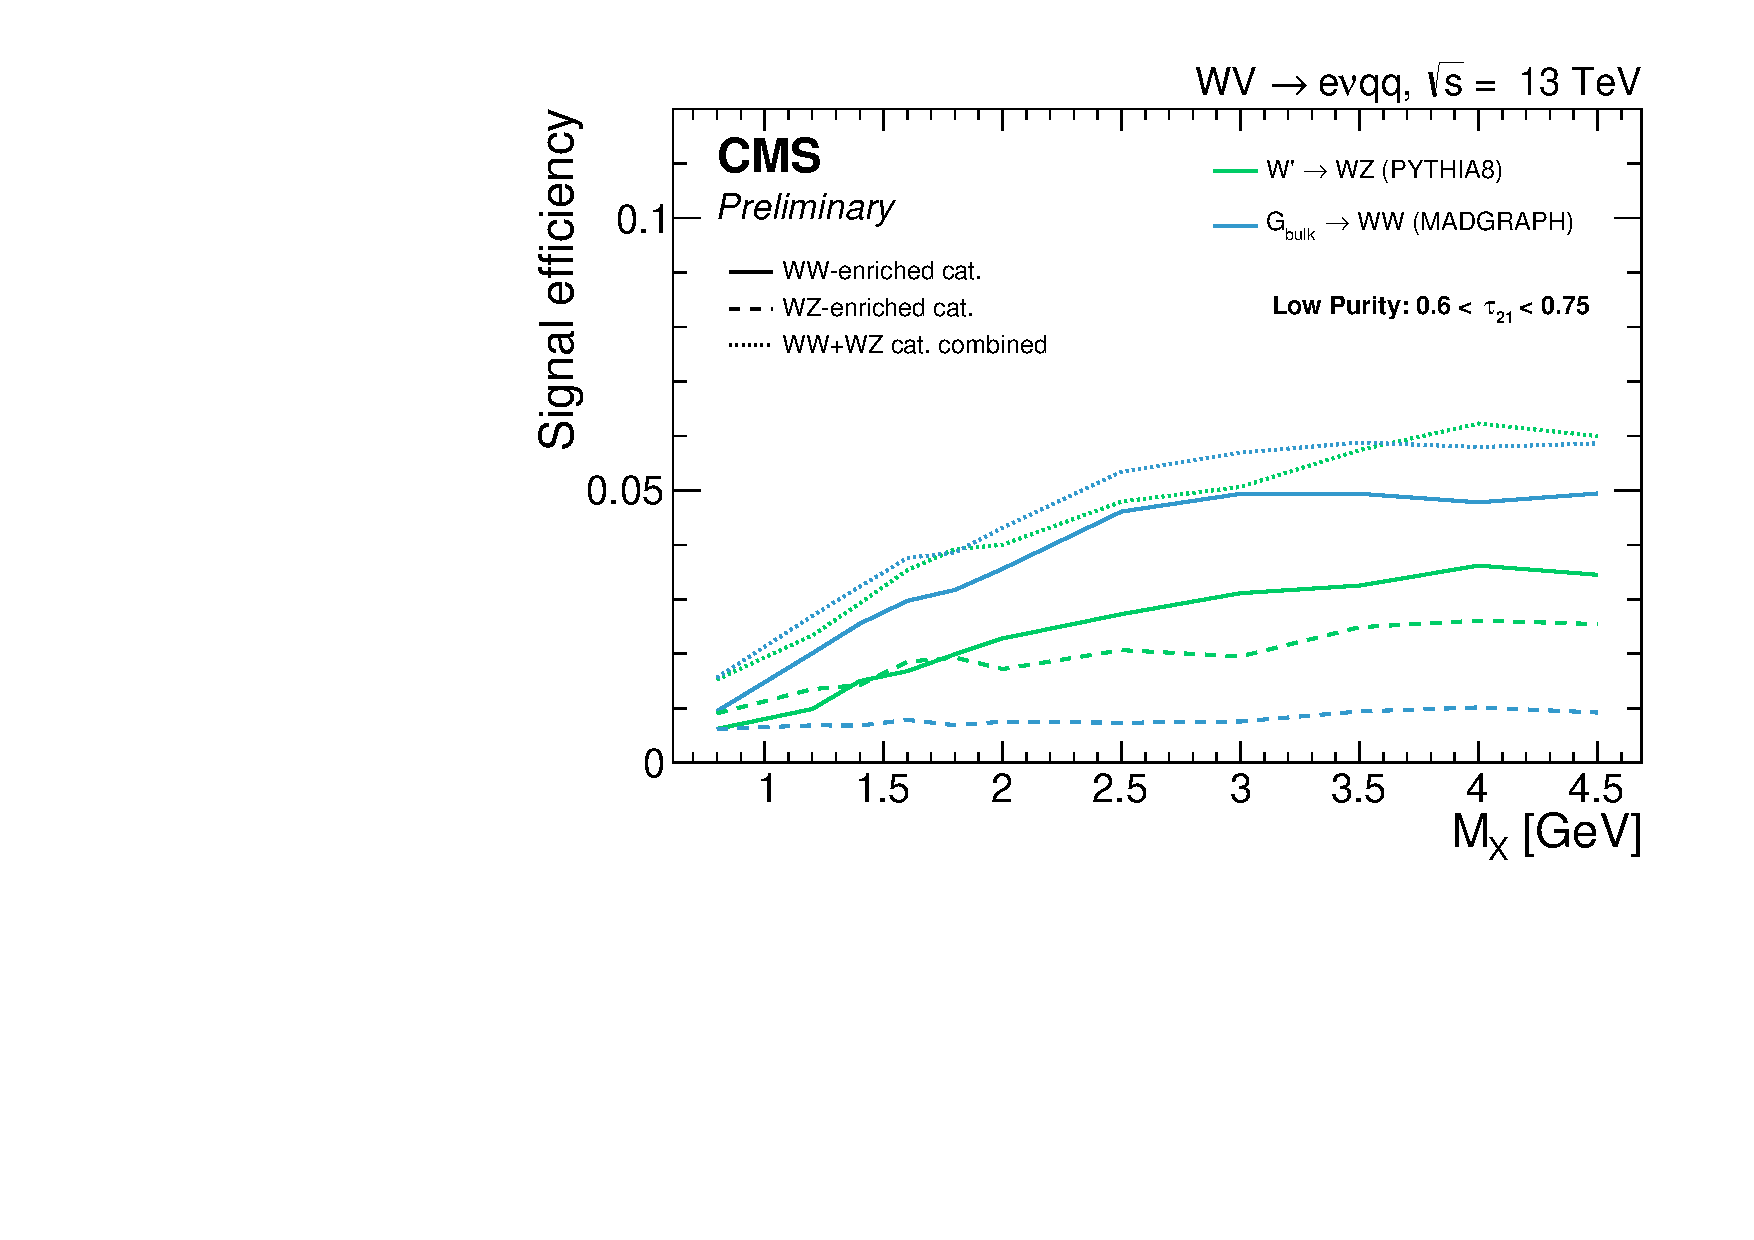
\includegraphics[width=0.48\textwidth]{\chten/WVanalysis/SignalEff/eff_LPV_el.pdf}\\
\caption{Expected signal efficiency for high-purity (top)
and low-purity (bottom) categories, in electron (left) and muon (right) channel separately,
for several resonance mass hypothesis. The efficiencies for the W-mass cut, the Z-mass cut
and for the mass categories combined are also shown.}
\label{fig:signaleff}
\end{figure}

%%%%%%%%%%%%%%%%%%%%%%%%%%%%%%%%%%%%%%
\section{Systematic uncertainties in the signal prediction}

%%%%%%%%%%%%%%%%%%%%%%%%%%%%%%%%%%%%%%
\section{Testing new resonance hypothesis}
\subsection{Profile likelihood procedure}
\subsection{The CL$_{s}$ method}
\subsection{Treatment of uncertainties}

%\section{Limits on the 8 and 13 TeV cross sections}
